\chapter{State of the Art\label{cha:chapter2}}

This chapter is intended to give an introduction about relevant terms, technologies and standards in the field of Semantic Web. It also delves into similar and related implementations (i.e. GAIA) to provide a comprehensive understanding of the current state of the art.

\section{Technologies \label{sec:tech}}

This section covers the fundamental technologies, specifically RDF and SPARQL, which serve as the foundational building blocks for structuring and querying data.

\subsection{RDF (Resource Description Framework)\label{sec:rdf_primer}}

The RDF is the foundation of the Semantic Web. It's a framework for describing resources on the Web thanks to URIs. A resource could be anything: a human being, a document, an object a concept \cite{rdf}. 
\\
\\
Specifically, RDF can be used to share and interlinked data. For example, if the following URI \space \textbf{http://www.example.org/bob\#me} is retrieved, it can provide information about Bob, such as his name, his age, and his friend.
If his friends' International Resource Identifiers (IRIs) are retrieved, like Alice's, more information regarding them can be accessed (i.e. more friends, interests, etc.). This process of "link navigation" is called Linked Data \cite{rdf}.
\\
\\
This RDF property can be useful for many use cases like: 
\begin{itemize}
	\item Creating distributed social networks by interlinking RDF descriptions of users.
	\item Integrating API feeds to ensure seamless discovery of additional data and resources by clients.
	\item Embedding machine-readable data into web pages.
	\item Standardizing data exchange across databases.
\end{itemize}

RDF interlinks resource with "statements". A statement is a triple containing a subject, a predicate, and an object.
The subject and the object stand for the resources that need to be represented. The predicate is the type of relation between those resources, and it is always phrased in one directional way (from the subject to the object). 
\\
This relation between the two is called a Property \cite{rdf}.
\\
It is possible to visualize these Triples as Graphs (see Figure \ref{fig:RDFTriple}) and query them using SPARQL.
\\
\\
In an RDF file, three type of data can  occur :IRIs, literals and blank nodes. 
\begin{itemize}
	\item IRIs are the identifiers of the resources. They are similar to the Uniform Resource Locators (URLs), but they don't provide information about where the resource is located or how to access it. They can only be used as mere identifiers. IRIs can appear in all three positions of a triple. 
	\item Literals are all the values that are not IRIs. They can be strings, numbers, dates, etc. They can only appear in the object position of a triple.
	\item Blank Nodes are all the nodes of a graph that are not identified by an IRI. They are like simple variables in algebra that represent something without saying what their value is. Blank nodes appear in the subject and object position of a triple. 
\end{itemize}
RDF allows grouping multiple RDF statements into multiple graphs and associate them with a single URI. 

\begin{lstlisting}[language=XML, caption={RDF Grouped Data}, label={lst:xml-rdf-grouped-example}, frame=single]
	<Bob> <is a> <person>.
	<Bob> <is a friend of> <Alice>.
	<Bob> <is born on> <the 4th of July 1990>.
	<Bob> <is interested in> <the Mona Lisa>.
\end{lstlisting}
One of the related problems with RDF is that the data model doesn't make assumptions about what resource URIs stand for.
For example the statement \space \textbf{ex:Apple ex:isLocated ex:California}, without any additional information about Apple, could be misleading. Without additional context Apple could refer to a fruit in California or Apple incorporated in Cupertino.
\\
One solution to this problem is to use IRIs in combinations with Vocabularies and other conventions that add semantic information about the resources.
\\
\\
In order to include Vocabularies in an RDF graph, RDF provides a Schema language.
\\
The RDF Schema allows the description of groups of related resources and the relations between them.
The class and property system is close to an object-oriented programming language. The difference with this model is that the RDF schema defines the properties in terms of Class and not vice versa as in object-oriented programming.
\begin{table}[h]
    \centering
    \begin{tabular}{lll}
        \toprule
        \textbf{Construct} & \textbf{Syntactic form} \\
        \midrule
        Class (a class) & C \texttt{rdf:type rdfs:Class}  \\
        Property (a class) & P \texttt{rdf:type rdf:Property} \\
        type (a property) & I \texttt{rdf:type C} \\
        subClassOf (a property) & C1 \texttt{rdfs:subClassOf C2} \\
        subPropertyOf (a property) & P1 \texttt{rdfs:subPropertyOf P2} \\
        domain (a property) & P \texttt{rdfs:domain C} \\
        range (a property) & P \texttt{rdfs:range C} \\
        \bottomrule
    \end{tabular}
    \caption{RDF Schema Constructs}
    \label{tab:rdf_schema_constructs}
\end{table}

An RDF Class is a group of resource with common characteristics. The resources in a class are referred to as instances of that class.
\\
\\
As discussed in previously, properties are used to describe the relations between subject and object resources.
The main properties for the construct of RDF schema are: 
\begin{itemize}
	\item \textbf{subClassOf} is used to state that all the instances of one class are instance of another.
	\item \textbf{subPropertyOf} is used to define that all resources related by one property are also related by another.
	\item \textbf{domain} is used to declare to which domain / class that property belong to.
	\item \textbf{range} is used to indicate the type of the property value.
\end{itemize}

RDF supports 4 main types of formats: The "Turtle family of RDFs", JSON-LD, RDF/XML and RDFa \cite{rdf}.


%  fix the citations.

\subsection{SPARQL \label{sec:bbb}}
In the RDF world, there are 2 main ways to retrieve data from an RDF store. The first one is to simple is to use a REST Endpoint and perform CRUD operations on the DB. This is in many cases the quickest solution, because it doesn't required new knowledge or new knowhow. 
The main problem is when the RDF store doesn't allow HTTP CRUD or doesn't provide a REST Endpoint.
In these cases the second solution is to use SPARQL.
\\
\\
SPARQL is a set of specifications that provide tools to retrieve and manipulate RDF graph content on the W3 or in an RDF store.
One of this tool is the SPARQL Query Language \cite{sparql}.
\\
\\
The SPARQL Query Language it's a query language, not far from the most well known SQL, is used for query formulation and retrieval of on the web.
\begin{lstlisting}[language=SPARQL, caption={Example of SPARQL Query}, basicstyle=\ttfamily, frame=single]
    PREFIX foaf: <http://xmlns.com/foaf/0.1/>
    SELECT ?name (COUNT(?friend) AS ?count)
    WHERE { 
        ?person foaf:name ?name . 
        ?person foaf:knows ?friend . 
    } GROUP BY ?person ?name
\end{lstlisting}

In order to make the exchange of query results among machines, SPARQL supports the following exchange formats: XML, JSON, CSV and TSV \cite{sparql}.



\section{Related Work \label{sec:tech}}

This section provides a detailed overview and analysis of the related work.

\subsection{GAIA (Automatic Instance Generator for Abox)}

The GAIA project, is a RDF triple generation tool developed by CEDAR. 
This research introduces an OWL-based generic RDF triple generator capable of loading any OWL ontology schema and generating compliant RDF instances, unlike the LUBM instance generator, which only supports its predefined LUBM ontology.
It strictly relies on OWL because the majority of ontologies that are currently available are written using this language \cite{raynaud2014gaia}.
\\
\\
GAIA is designed for performance and scalability, thanks to the multithreading implementation that allows to generate a large volume of triples, making it perfect for ontology benchmarking or synthetic dataset generation \cite{raynaud2014gaia}.
\\
\\
Despite its performance and accuracy, GAIA has several limitations. The software is missing a schema visualization system or interactive graph explorer. This makes it hard for a human to visualize at glance the newly generated instances.
The system is also not limited to machines with JAVA installed on it, and having it implemented as IDE extension is a very challenging task due to its architecture.
\\
Furthermore, GAIA does not natively support RDF Schema (RDFS) or lightweight RDF graphs in Turtle or JSON-LD format (it only supports $.RDF$ or $.XML$).

\begin{lstlisting}[language=XML, caption={Example of RDF/XML Data}, basicstyle=\ttfamily\footnotesize, frame=single]
    <?xml version="1.0" encoding="UTF-8"?>
    <rdf:RDF xmlns:rdf="http://www.w3.org/1999/02/22-rdf-syntax-ns#"
             xmlns:owl="http://www.w3.org/2002/07/owl#"
             xmlns:rdfs="http://www.w3.org/2000/01/rdf-schema#"
             xmlns:ex="http://example.org/"
             xml:base="http://example.org/ontology"
             xmlns:xsd="http://www.w3.org/2001/XMLSchema#">

        <owl:Ontology rdf:about="http://example.org/ontology">
            <owl:versionInfo>1.0</owl:versionInfo>
        </owl:Ontology>

        <rdf:Description rdf:about="http://example.org/Class/Person">
            <rdf:type rdf:resource="http://www.w3.org/2002/07/owl#Class"/>
            <rdfs:label>Person</rdfs:label>
        </rdf:Description>

        <rdf:Description rdf:about="http://example.org/Class/Organization">
            <rdf:type rdf:resource="http://www.w3.org/2002/07/owl#Class"/>
            <rdfs:label>Organization</rdfs:label>
        </rdf:Description>

        <rdf:Description rdf:about="http://example.org/Individual/JohnDoe">
            <rdf:type rdf:resource="http://example.org/Class/Person"/>
            <ex:name>John Doe</ex:name>
        </rdf:Description>

        <rdf:Description rdf:about="http://example.org/Individual/AcmeCorp">
            <rdf:type rdf:resource="http://example.org/Class/Organization"/>
            <ex:name>Acme Corporation</ex:name>
        </rdf:Description>

    </rdf:RDF>
\end{lstlisting}

\begin{figure}[H]
    \centering
    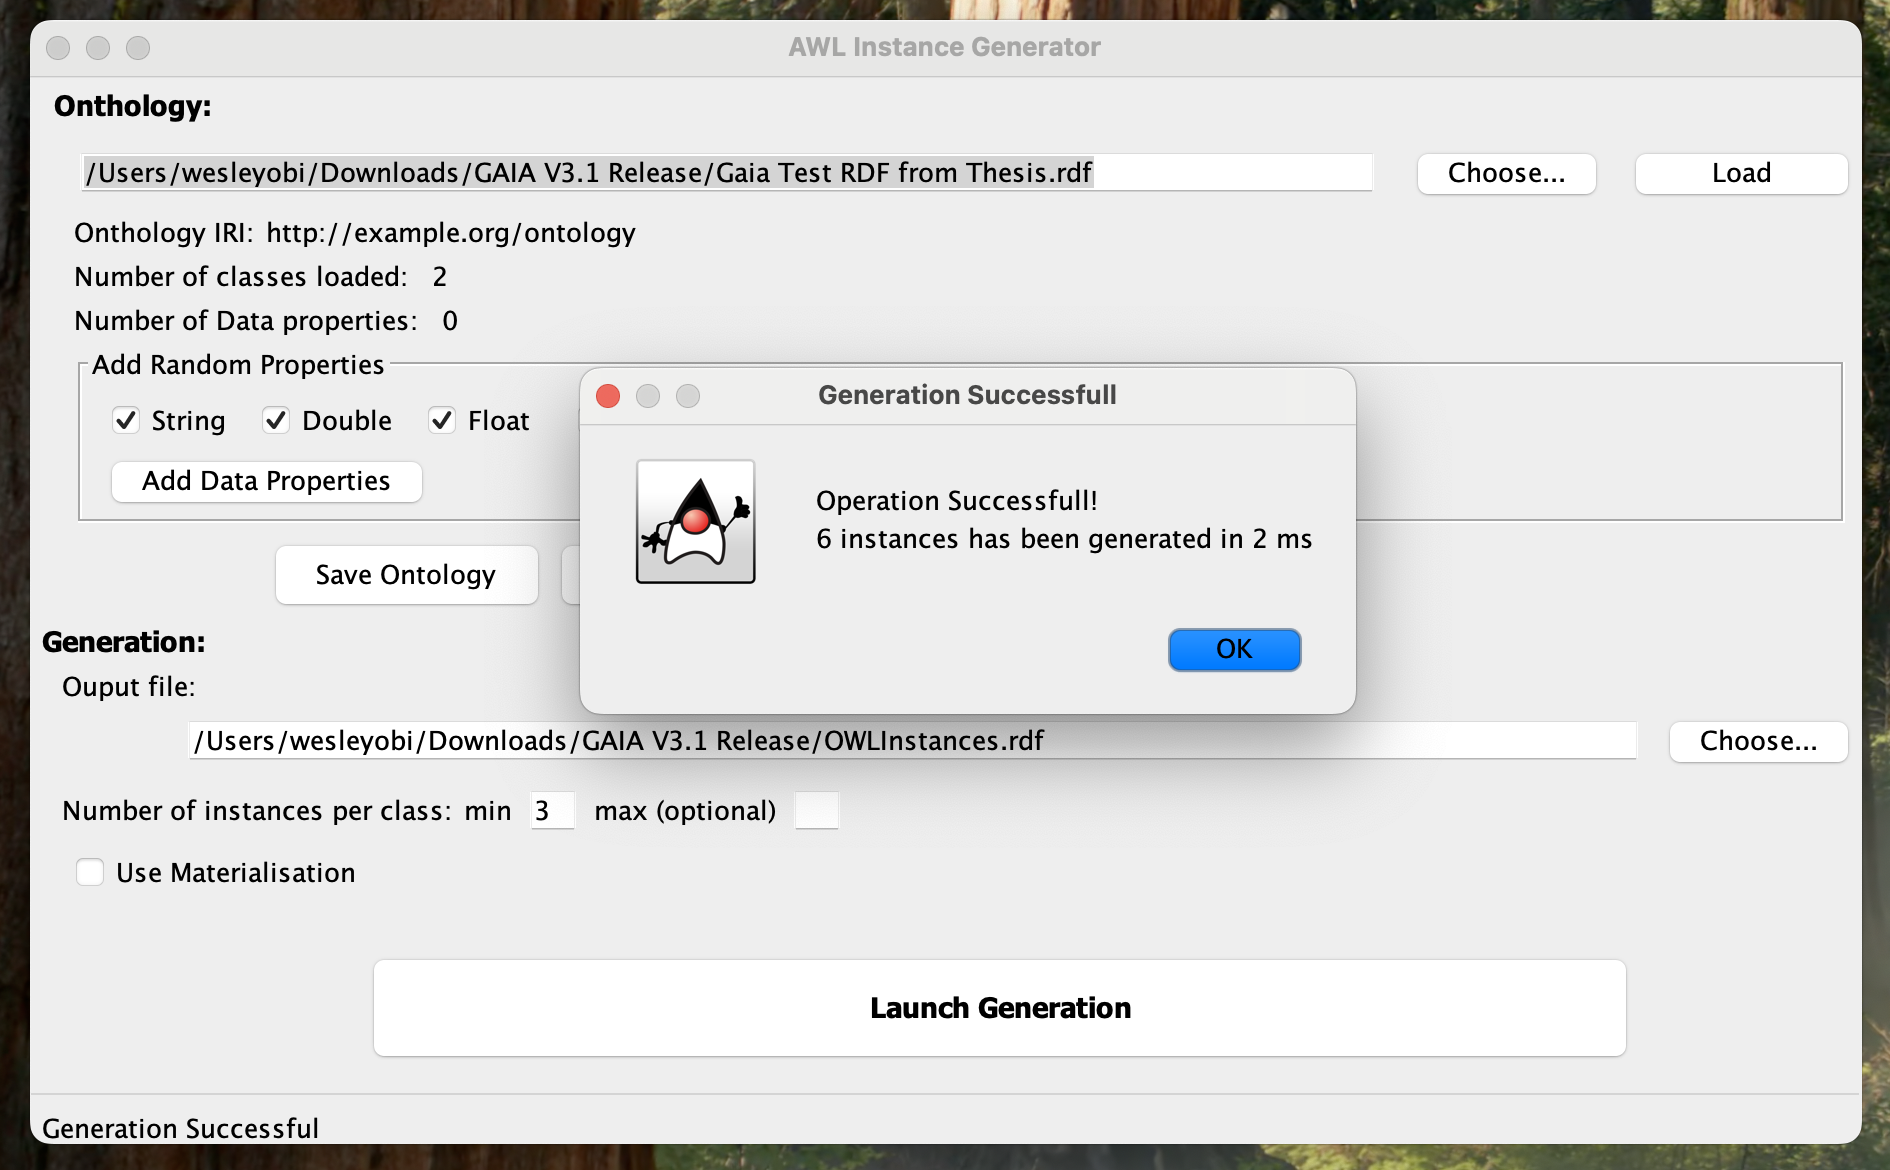
\includegraphics[width=13cm]{GAIA.png}\\
    \caption{GAIA Instance Generator used via GUI}\label{fig:gaia}
  \end{figure}

  \begin{lstlisting}[language=XML, caption={Results of RDF/XML generated instances}, basicstyle=\ttfamily\footnotesize, frame=single]
    ...
    <!-- Instances Generated by OWL_GENERATOR -->

    <owl:NamedIndividual rdf:about="http://example.org/ontology#Organization_instance0">
        <rdf:type rdf:resource="http://example.org/ontology#Organization"/>
    </owl:NamedIndividual>

    <owl:NamedIndividual rdf:about="http://example.org/ontology#Organization_instance1">
        <rdf:type rdf:resource="http://example.org/ontology#Organization"/>
    </owl:NamedIndividual>

    <owl:NamedIndividual rdf:about="http://example.org/ontology#Organization_instance2">
        <rdf:type rdf:resource="http://example.org/ontology#Organization"/>
    </owl:NamedIndividual>

    <owl:NamedIndividual rdf:about="http://example.org/ontology#Person_instance0">
        <rdf:type rdf:resource="http://example.org/ontology#Person"/>
    </owl:NamedIndividual>

    <owl:NamedIndividual rdf:about="http://example.org/ontology#Person_instance1">
        <rdf:type rdf:resource="http://example.org/ontology#Person"/>
    </owl:NamedIndividual>

    <owl:NamedIndividual rdf:about="http://example.org/ontology#Person_instance2">
        <rdf:type rdf:resource="http://example.org/ontology#Person"/>
    </owl:NamedIndividual>

    </rdf:RDF>
\end{lstlisting}

\subsection{The instance Generator project suggested by the professor}
...

\subsection{RDF Graph Preview}

The Graph RDF Graph Preview it's an open source project developed by Lucien Reboul \cite{rdfpreview2022}.
\\
It's a VSCode extension that allows to load RDF files and visualize them as graphs. It uses the D3.js library as core graph rendering system.
\\
\\
One advantage of this extension is that it allows to quickly visualize RDF graph without leaving the current workspace. 
\\
But unfortunately, this plugin is only able to render RDF files written Turtle and N-Triples/N3 formats. The tool provides no support for automatic instance generation, forcing users to do all the heavy work manually.
\\
\\
\begin{figure}[htb]
    \centering
    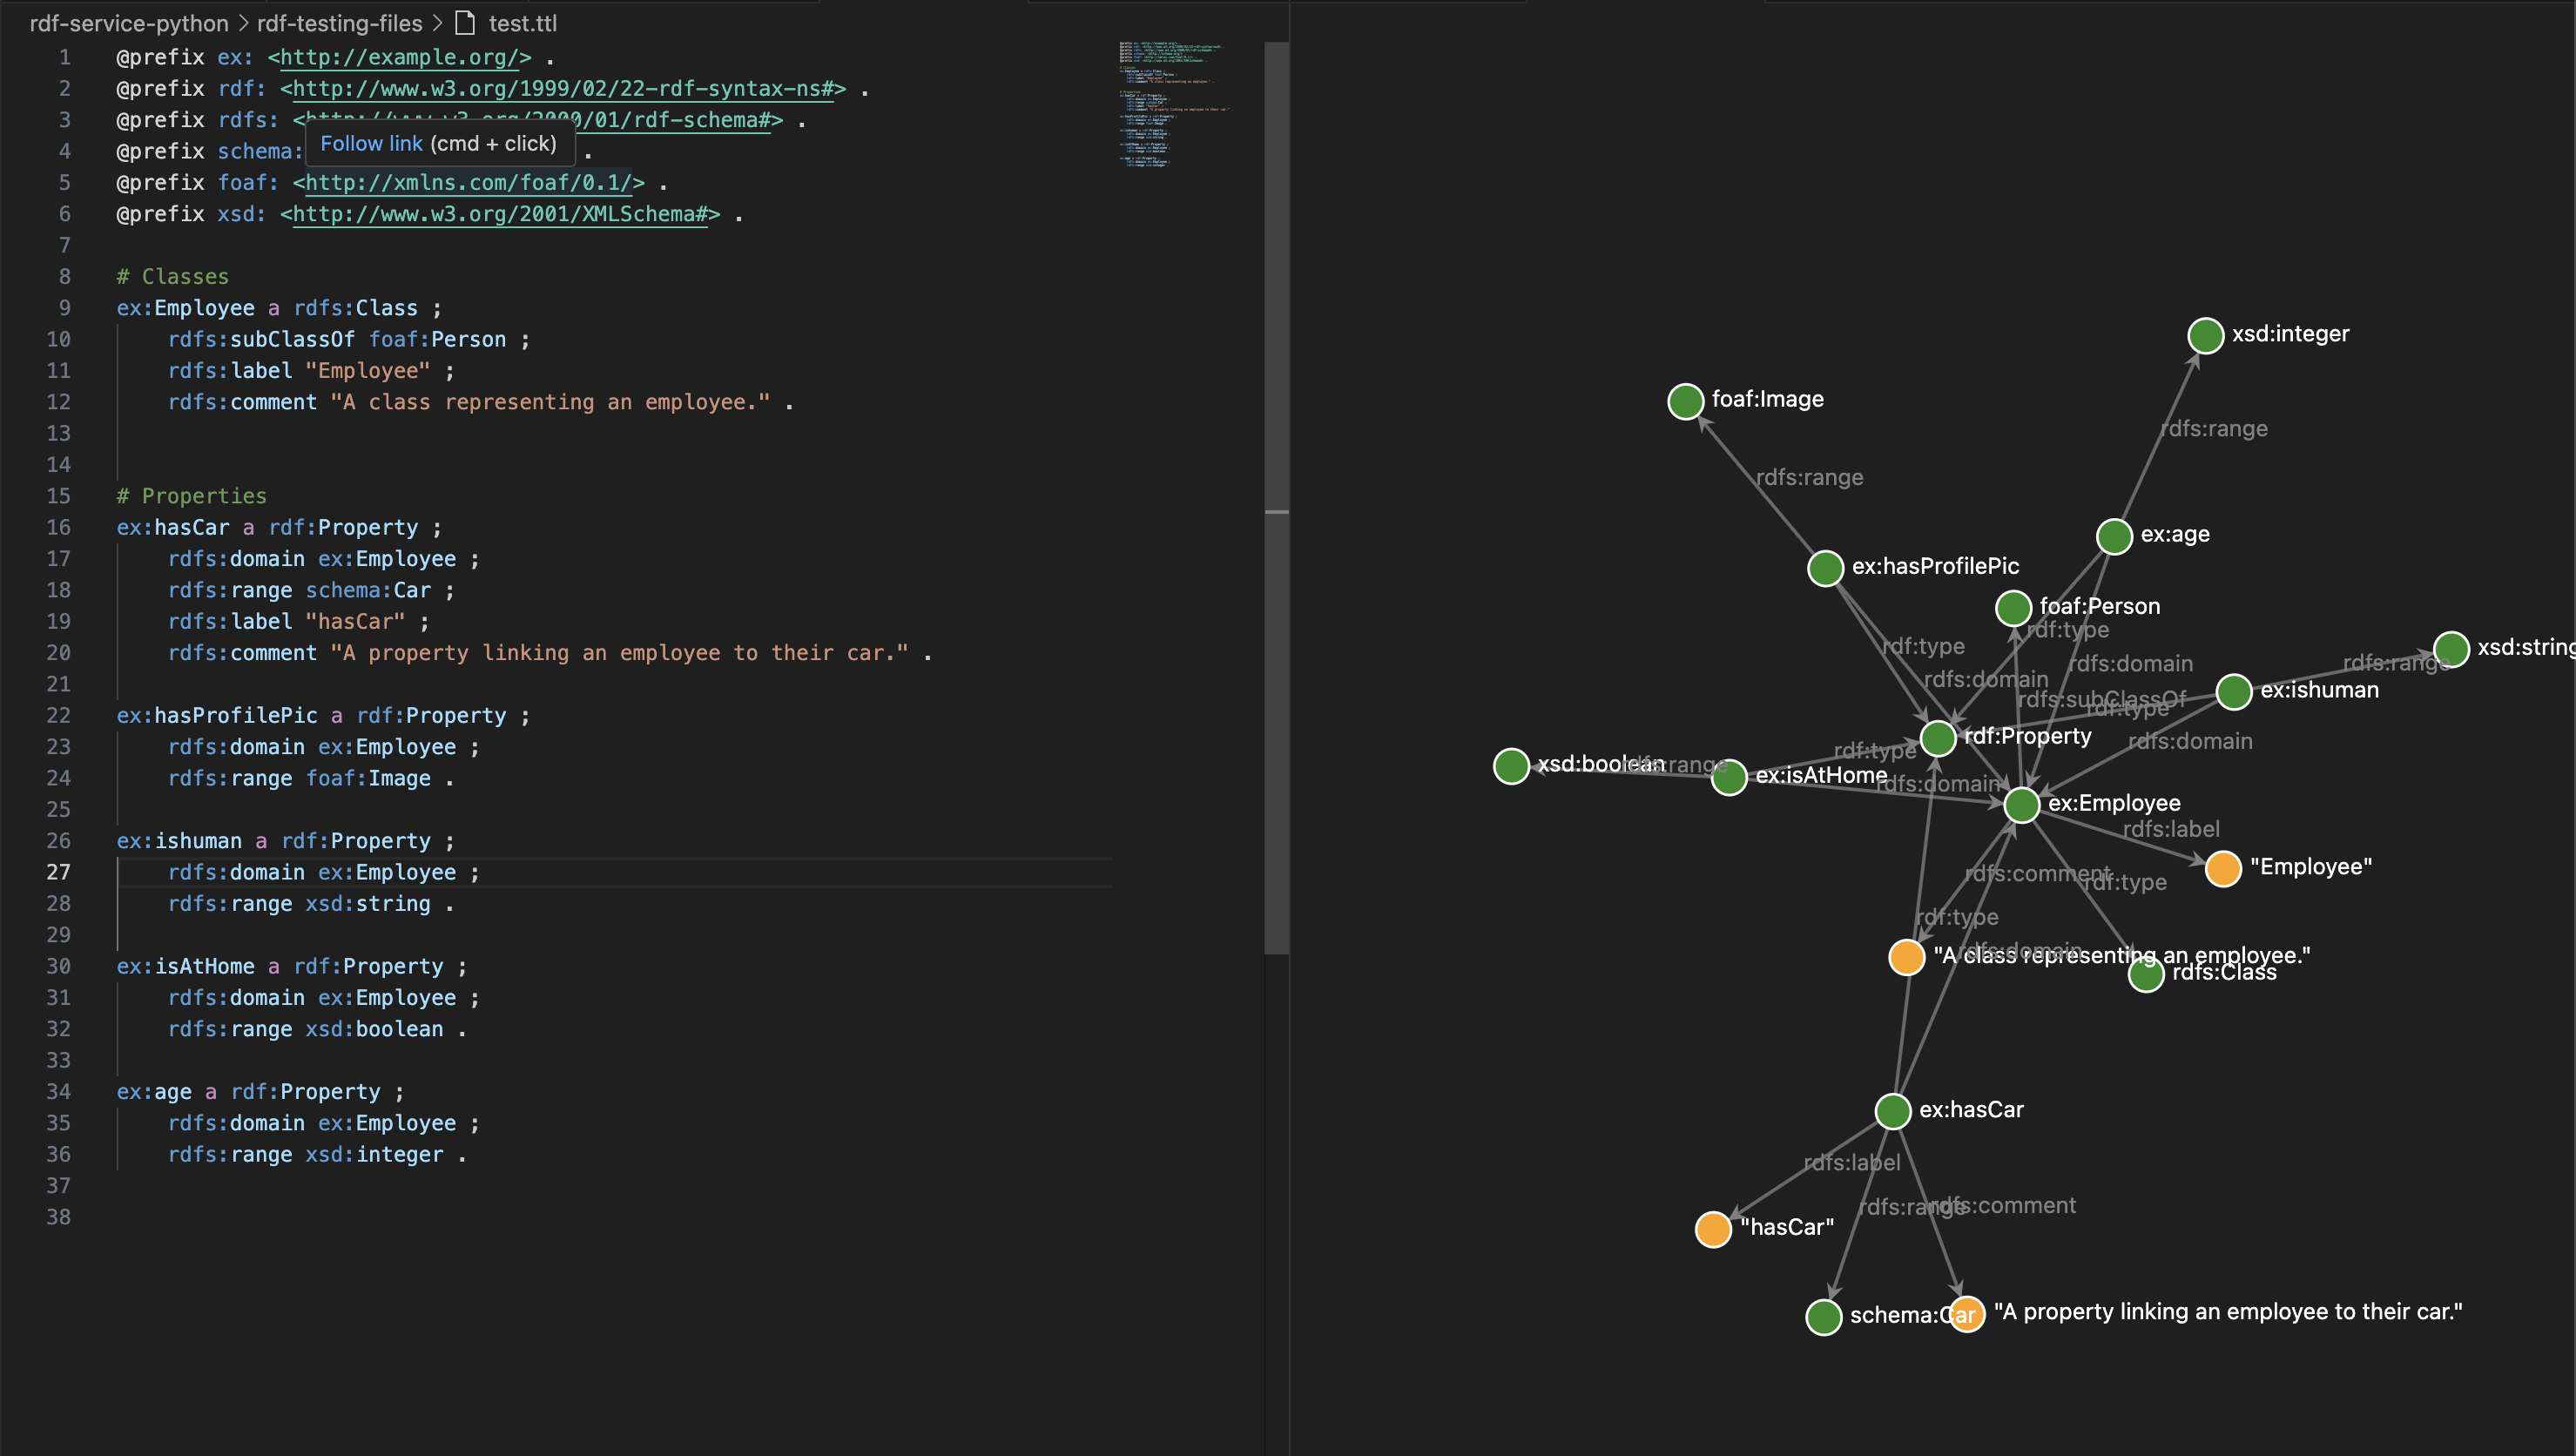
\includegraphics[width=13cm]{RDFPreviewExtension.png}\\
    \caption{RDF Graph Preview VSCode Extension}\label{fig:RDFPreviewExtension}
  \end{figure}
  

% write about  another RDF instance generation project,
% the ontodia maybe? 
% also protégé 